\newpage

\subsubsection{Границе}\label{sssec:superstar}

\zadatak
Докажи да важи неједнакост
\begin{equation}
    \okvir{1-\frac1x \le \ln x \le x - 1},
\end{equation}
којом се дефинишу {\sl доња\/} и {\sl горња\/} граница природног логаритма.

\resenje
Погледајмо прво десни део неједнакости. Ако дефинишемо функцију
$$
y=\ln x - (x - 1),
$$
потребно је да докажемо да је $y\le0$ за свако $x>0$.
Интуитивно је јасно да тврђење важи, јер $\ln x$ много спорије расте од $x-1$,
и формални доказ ће нам се заснивати на томе.

Први \idx{извод} функције~је
$$
y' = \frac1x - 1,
$$
који има јединствену нулу $y'=0$ za $x=1$, где је и $y=0$. Како је други извод
$$
y''=-\frac1{x^2}<0,
$$
увек негативан, то значи да функција $y$ нема {\sl превојних тачака\/} и да тачка $(1,0)$ 
представља {\sl\idx{максимум}\/} функције  $y$,
одакле је $y\le0$, односно,
$$
\ram{\ln x \le x - 1}.
$$

Ако у ову неједнакост уместо $x$ ставимо $1/x$, можемо писати
\begin{align*}
    \ln(1/x) &\le \frac1x -1 \\
    -\ln x &\le \frac1x -1, 
\end{align*}
где, када изрази замене стране и знак, добијамо
$$
    \ram{1-\frac1x \le \ln x},
$$
што представља леви део неједнакости из задатка.\hfill\QED\QEDidx

\definecolor{darkgreen}{HTML}{00AA00}

\dodatak 
Све три функције из неједнакости се {\sl додирују\/} у тачки $(1,0)$, што значи да
у тој тачки све три имају исту {\sl тангенту}, односно, исти први извод $y'(1)=1$;
иначе би се секле и неједнакост не би важила.

$$
\slika{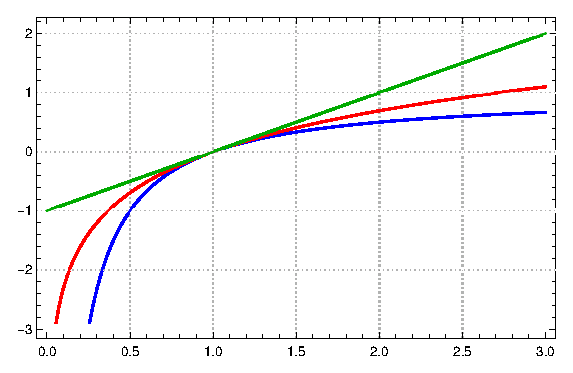
\includegraphics[width=80mm]{eps/royal.eps}}{$y=
{\color{blue}1-1/x};\
{\color{red}\ln x};\
{\color{darkgreen}x-1}
.$}
$$


\newpage
